\documentclass[handout]{beamer}

% math packages
\usepackage{amssymb}

% theme
\usetheme{Rochester}
\usecolortheme{dove}
\usefonttheme{default}

% make the title BIG
\setbeamerfont{title}{series=\bfseries,size=\Huge, parent=structure}

% remove the side title header
\setbeamertemplate{headline}{}

%gets rid of bottom navigation bars
\setbeamertemplate{footline}{}

%gets rid of navigation symbols
\setbeamertemplate{navigation symbols}{}

% define "head" commands for transitions
\newcommand{\headone}{\centering \bf \Huge}
\newcommand{\headtwo}{\centering \bf \LARGE}
\newcommand{\headthree}{\centering \bf \Large}

% define a "spaceit" command for spacing between paragraphs
\newcommand{\spaceit}{\vspace{10mm}}

% define a "red" command to make text red.
\newcommand{\red}[1]{\textcolor{red}{#1}}
\newcommand{\blue}[1]{\textcolor{blue}{#1}}


% simply the style of the lists
\setbeamertemplate{itemize items}[default]
\setbeamertemplate{enumerate items}[default]

% increase the default spacing between equations
\setlength{\jot}{5pt}

% custom color for "blockcode"
\usepackage{fancyvrb,color}

\DefineVerbatimEnvironment{blockcode}
  {Verbatim}
  {formatcom=\color{blue}}


\begin{document}
\title{Modeling Binary Outcomes: Part 1}   
\author{Carlisle Rainey} 
\date{} % remove date 

\frame{\titlepage} 

\frame{
\textbf{Binary Outcomes}
\begin{itemize}
\pause \item Binary outcomes are categorical outcome variables with exactly two categories, such as whether or not someone voted, whether two countries are at war, and so on. 
\pause \item These variables are usually coded as $y_i \in \{0, 1\}$, with one representing ``an event'' and zero representing ``a non-event.''
\pause \item In generic language, we'll say that $y_i = 1$ means that "an event has occurred" and $y_i = 0$ means that "an event has not occurred." 
\pause \item This allows us to talk about the ``probability of an event.''
\end{itemize}
}

\frame{
\headone
Linear Probability Model (LPM)
}

\frame{
We can use the normal-linear model (i.e., OLS) with binary outcome variables.
\begin{itemize}
\pause \item Recall that we the linear model is represented by the equation $E(y_i) = X_i\beta$. 
\pause \item It is important to note that a probability is just a particular kind of expected value--a probability is an expected value of a binary variable. 
\pause \item Since $y_i$ is binary, the $E(y_i) = Pr(y_i)$, giving us $Pr(y_i) = X_i\beta$.
\end{itemize}
}

\frame{
\textbf{Advantages of the LPM}
\begin{itemize}
\pause \item It is \underline{very} easy to estimate (i.e., OLS; $\hat{\beta} = (X'X)^{-1}X'y$).
\pause \item It is easy to interpret (i.e., a one unit change in $x_j$ leads to a $\hat{\beta_j}$ unit increase in $Pr(y)$).
\end{itemize}
}

\frame{
\headone
Disadvantages of the LPM
}

\frame{
\textbf{Unbounded predictions.}\\\vspace{5mm}
\begin{itemize}
\pause \item Because the potential values for the explanatory variables are unbounded, you can obtain predicted probabilities above one and below zero. 
\pause \item Of course, these predictions make no sense.
\end{itemize}
}

\frame{
\textbf{Conditional heteroskedasticity.}\\\vspace{5mm}
\begin{itemize}
\pause \item The normal-linear model assumes a constant variance. 
\pause \item However, it is impossible to have homoskedastic residuals of a binary outcome if the probability of an event varies. \pause \item Specifically, if $y_i$ is binary, then $var(y_i) = Pr(y_i)[1 - Pr(y_i)]$, which, for the LPM, equals $X_i\beta(1 - X_i\beta)$. 
\pause \item You'll notice that non-zero coefficients imply heteroskedasticity.
\end{itemize}
}

\frame{
\textbf{Non-normal errors.}\\\vspace{5mm}
\begin{itemize}
\pause \item Normal errors implies that the residuals can take on any value along the real line, with values closer to zero being more likely and errors outside three standard deviations being quite unlikely. 
\pause \item However, if $y_i$ is binary, then the residual can take on only two values: $-Pr(y_i)$ or $1 - Pr(y_i)$.
\end{itemize}
}

\frame{
\textbf{Functional form.}\\\vspace{5mm}
\begin{itemize}
\pause \item Theoretically, you'd probably expect explanatory variables to have smaller effects as $Pr(y_i)$ approaches zero or one. 
\pause \item The LPM assumes that the effects are constant.
\end{itemize}
}

\frame{
\headtwo
We need a model that better matches our substantive understanding of the process.
}

\frame{
We know our generic model.
\begin{huge}
\begin{equation*}
\pause Y \sim f(y | \theta)
\end{equation*}
\end{huge}
Questions:
\begin{enumerate}
\pause \item What distribution $f$ should we choose for our binary outcome? \pause \red{The Bernoulli distribution makes sense.}
\pause \item If we choose Bernoulli, what does $\theta$ look like? \pause \red{$\theta = \pi \in [0, 1]$.}
\end{enumerate}
}

\frame{
\headone Building in Covariates\\\vspace{5mm}
\pause \headthree the inverse\footnote{You might wonder why we work with an inverse function. There is a long answer to that, but the short answer is that people started off writing their models as $g(\theta_i) = X_i\beta$. We can easily go from $g$ to $g^{-1}$ and back. However, it is easiest to work with $g^{-1}$ (i.e., the \textit{inverse} link function), so that's what we'll use primarily. Authors sometimes get a little lax in their language and use "link function" to refer to an inverse link function. This is not technically correct, but it should be clear from the context what they mean.} link function $g^{-1}$
}

\frame{
For the normal-model, we modeled the mean using $\mu = X_i\beta$.\\\vspace{5mm}
\pause Maybe we could try something similar for the Bernoulli model.\\\vspace{5mm}
\pause Perhaps $\pi_i = X_i\beta$? \pause \red{$X_i\beta$ is not properly bounded.}
}

\frame{
\begin{Large}
Generic Facts: 
\begin{enumerate}
\pause \item $X_i\beta \in \mathbb{R}$
\pause \item $\theta \in \Theta \subseteq \mathbb{R}$
\end{enumerate}\vspace{5mm}
\end{Large}
\pause What we need:
\begin{enumerate}
\pause \item A \textbf{link function} $g$ that maps $\Theta$ to $\mathbb{R}$ (i.e., $g: \Theta \rightarrow \mathbb{R}$)
\pause \item Or an \textbf{inverse-link function} $g^{-1}$ that maps $\mathbb{R}$ to $\Theta$ (i.e., $g^{-1}: \mathbb{R} \rightarrow \Theta$).
\end{enumerate}\vspace{5mm}
\pause It's usually a little easier to work with the inverse-link function than the link function.
}

\frame{
\begin{Large}
Generic Facts: 
\begin{enumerate}
\pause \item $X_i\beta \in \mathbb{R}$
\pause \item $\pi \in [0, 1] \subseteq \mathbb{R}$
\end{enumerate}\vspace{5mm}
\end{Large}
\pause What we need:
\begin{enumerate}
\pause \item A \textbf{link function} $g$ that maps $[0, 1]$ to $\mathbb{R}$ (i.e., $g: [0, 1] \rightarrow \mathbb{R}$)
\pause \item Or an \textbf{inverse-link function} $g^{-1}$ that maps $\mathbb{R}$ to $[0, 1]$ (i.e., $g^{-1}: \mathbb{R} \rightarrow [0, 1]$).
\end{enumerate}\vspace{5mm}
\pause What sort of function maps the real link to $[0, 1]$? \red{cdfs?}
}

\frame{
We might choose to use the cdf of the \textit{logistic} distribution $F(x) = \Lambda(x) = \dfrac{1}{1 + e^{-x}}$. \pause This is \blue{\texttt{plogis()}} in R.\vspace{5mm}

\pause For $X_i\beta \in \mathbb{R}$\pause, $g^{-1}(X\beta) \pause  = \Lambda(X_i\beta) \in [0, 1]$. \pause This is exactly what we want--a ``logit model'' or ``logistic regression model.''\\\vspace{5mm}
Ways to write:
\begin{enumerate}
\pause \item $Y_i \sim \text{Bernoulli}(\pi_i)$, where $\pi_i = \Lambda(X_i\beta) = \frac{1}{1 + e^{-X_i\beta}}$\\\vspace{3mm}
\pause \item $\text{Pr}(Y_i = 1) = \frac{1}{1 + e^{-X_i\beta}}$\\\vspace{3mm}
\pause \item $\text{Pr}(Y_i = 1) = \text{logit}^{-1}(X_i\beta)$
\pause \item $\text{logit}(\pi_i) = X_i \beta$
\end{enumerate}
}

\frame{
\begin{Large}
\textbf{Maximum Likelihood Estimation}
\end{Large}
\begin{enumerate}
\pause \item Write down a probability model.
\pause \item Find the probability of the data given the parameters--the likelihood function.
\pause \item Take the log and simplify.
\pause \item Maximize.
	\begin{itemize}
	\pause \item Analytically. (Usually difficult or impossible.)
	\pause \item Numerically. (Usually easier.)
	\end{itemize}
\end{enumerate}
}

\frame{
\begin{Large}
Step 1: Write down a probability model.\\\vspace{5mm}
\end{Large}
\begin{center}
$Y_i \sim \text{Bernoulli}(\pi_i)$, where $\pi_i = \Lambda(X_i\beta) = \frac{1}{1 + e^{-X_i\beta}}$\
\end{center}
}

\frame{
\begin{Large}
Step 2: Find the probability of the data given the parameters--the likelihood function.\\\vspace{5mm}
\end{Large}
\pause First, note the probability of a single observation: $\text{Pr}(y_i) = \pi_i^{y_i}(1 - \pi_i)^{1 - y_i}$.\\\vspace{5mm}
\pause Then, assuming independence, we can get the probability of the data: $\text{Pr}(y | \beta) =  \mathcal{L}(\beta | y) = \prod_{i = 1}^n \pi_i^{y_i}(1 - \pi_i)^{1 - y_i}$. \pause For simplicity, we'll just remember that $\pi_i = \Lambda(X\beta)$.
}

\frame{
\begin{Large}
Step 3: Take the log and simplify.\\\vspace{5mm}
\end{Large}
\begin{equation*}
\begin{aligned}
\pause \mathcal{L}(\beta | y) &= \prod_{i = 1}^n \pi_i^{y_i}(1 - \pi_i)^{1 - y_i}\\
\pause \log \mathcal{L}(\beta | y) &= \sum_{i = 1}^n \log \pi_i^{y_i}(1 - \pi_i)^{1 - y_i}\\
\pause \log \mathcal{L}(\beta | y) &= \sum_{i = 1}^n y_i \log \pi_i + \sum_{i = 1}^n (1 - y_i)\log(1 - \pi_i)\\
\pause \log \mathcal{L}(\beta | y) &= \sum_{i = 1}^n y_i \log \Lambda(X_i\beta) + \sum_{i = 1}^n (1 - y_i)\log\left[1 - \Lambda(X_i\beta)\right]
\end{aligned}
\end{equation*}
}

\begin{frame}[fragile]
\begin{Large}
Step 4: Optimize\\\vspace{3mm}
\end{Large}
\begin{footnotesize}
\begin{blockcode}
# define log-likelihood function
ll.logit <- function(beta, y, X) {
  p <- plogis(X%*%beta)
  loglik <- sum(y*log(p)) + sum((1 - y)*log(1 - p))
  return(loglik)
}

# optimize
logit <- function(y, X) {
  init.par <- rep(0, ncol(X))
  est <- optim(par = init.par, fn = ll.logit, y = y, X = X,
               control = list(fnscale = -1),
               hessian = TRUE)  # return the hessian
  if (est$convergence != 0) print("Model did not converge!")
  beta.hat <- est$par
  cov <- solve(-est$hessian)
  res <- list(beta.hat = beta.hat,
              cov = cov)
  return(res)
}
\end{blockcode}
\end{footnotesize}
\end{frame}

\begin{frame}[fragile]
\begin{Large}
Test our function\\\vspace{3mm}
\end{Large}
\begin{blockcode}
# generate fake data
n <- 1000
x1 <- rnorm(n)
x2 <- rnorm(n)
X <- cbind(1, x1, x2)
b <- c(1, -1, 2)
p <- plogis(X%*%b)
y <- rbinom(n, 1, p)

# estimate model
m1 <- logit(y, X)  # our function
m2 <- glm(y ~ x1 + x2, family = "binomial")
\end{blockcode}
\end{frame}

\begin{frame}[fragile]
\begin{Large}
Fearon and Laitin (2003)\\\vspace{3mm}
\end{Large}
\begin{footnotesize}
\begin{blockcode}
# load packages
library(foreign)  # for read.dta()
library(arm)  # for display()

# load data
fl <- read.dta("http://crain.co/am-files/data/fearon-laitin.dta")

# something weird is going on
table(fl$onset)  # wtf?
fl$onset[fl$onset == 4] <- 1 # recode weird case

# estimate model
m <- glm(onset~ warl + gdpenl + lpopl1 + 
           lmtnest + ncontig + Oil + nwstate + 
           instab + polity2l + ethfrac + relfrac, 
         family = binomial, data = fl)

# display estimates
display(m) # replicated!
\end{blockcode}
\end{footnotesize}
\end{frame}

\begin{frame}[fragile]
\begin{columns}[T] % align columns
\begin{column}{.48\textwidth}
% left part
\begin{verbatim}
            coef.est coef.se
(Intercept) -6.73     0.74  
warl        -0.95     0.31  
gdpenl      -0.34     0.07  
lpopl1       0.26     0.07  
lmtnest      0.22     0.08  
ncontig      0.44     0.27  
Oil          0.86     0.28  
nwstate      1.71     0.34  
instab       0.62     0.24  
polity2l     0.02     0.02  
ethfrac      0.17     0.37  
relfrac      0.29     0.51  
---
  n = 6327, k = 12
\end{verbatim}

\end{column}%
\hfill%
\begin{column}{.48\textwidth}
% right part
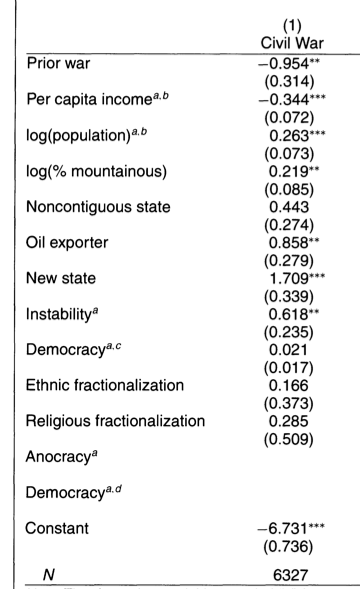
\includegraphics[scale = .38]{figs/fearon-laitin-coefs.png}
\end{column}%
\end{columns}
\end{frame}
\end{document}

\end{document}
